\mysubsection{Fonctionnement d'un ordinateur}

\ifbook{

  \mysubsubsection{Fonctionnement schématique d'un ordinateur}

  \paragraph{} Avant d'entrer dans le coeur du sujet, il est nécessaire de tout d'abord bien
  comprendre comment fonctionne la brique la plus élémentaire de tout système informatique:
  l'ordinateur.

  \begin{figure}[hb]
    \begin{center}
      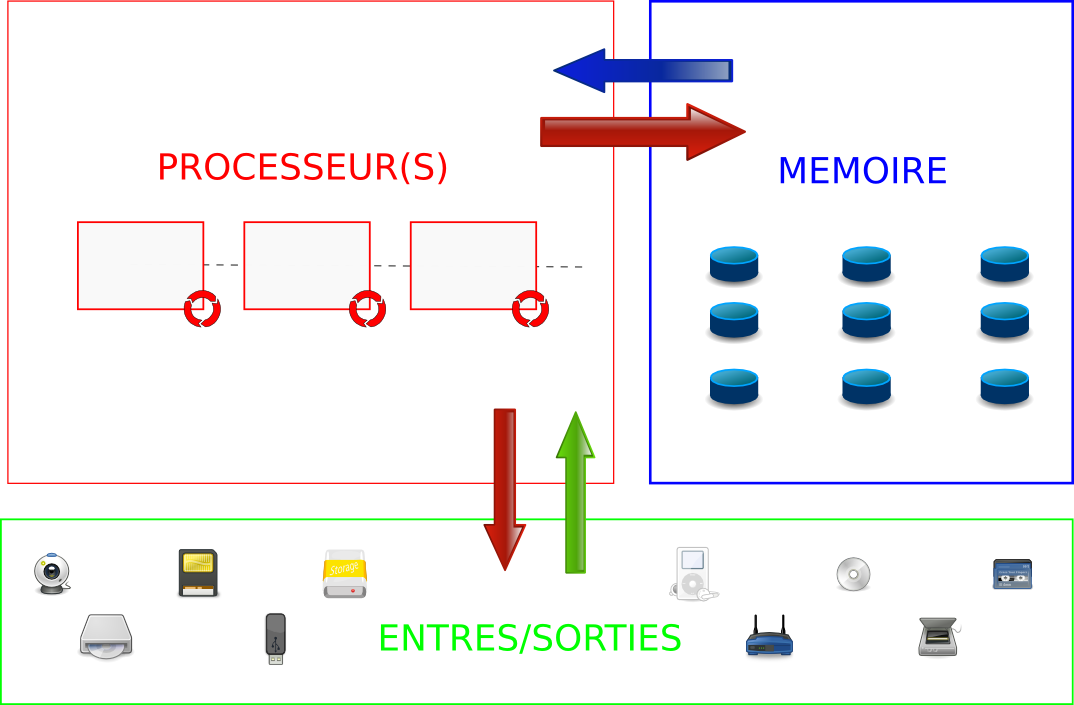
\includegraphics[scale=0.3]{img/cpu-schematics.png}
      \caption{Schéma simplifié du fonctionnement d'un ordinateur}
      \label{schema-ordi}
    \end{center}
  \end{figure}

  \paragraph{} Comme l'illustre le dessin \ref{schema-ordi} (page \pageref{schema-ordi}), un
  ordinateur, aussi complexe soit-il peut être résumé aux trois composants suivants:
  \begin{description}
    \item[Processeur] unité de traitement de l'ordinateur, c'est lui qui réalise les calculs et qui
    produit les résultats ;
    \item[Mémoire] espace de travail du processeur, la mémoire lui permet de stocker les résultats,
    intermédiaires ou finaux, de ses calculs ;
    \item[Entrées/Sorties] pour communiquer avec le "monde extérieur" (clavier, écran, disques durs,
    réseaux,...) le processeur dispose de différents composants matériels dédiés aux différentes
    entrées/sorties.
  \end{description}

  \paragraph{Distinction mémoire vive et mémoire morte} Sans rentrer dans les détails techniques, il
  est important de noter que les périphériques de stockage, tels que les disques durs, ne sont pas 
  conceptuellement très différents de la mémoire. Dans les deux cas, ils permettent au processeur de 
  stocker des résultats.

  \paragraph{Distinction des types de mémoires} Il existe différents types de mémoires qui peuvent 
  être séparées selon qu'elles sont rapide ou lente : plus la mémoire est "proche" du processeur, 
  plus elle est rapide. Nous avons donc par ordre décroissant de vitesse : 

  \begin{itemize}
    \item la RAM,
    \item le disque dur,
    \item le stockage sur une machine distincte.
  \end{itemize}

  \paragraph{Distinction mémoire vive et mémoire morte}  En outre, il faut noter qu'une mémoire 
  \textbf{volatile} a besoin d'électricité pour être conservée, à la différence du \textbf{stockage 
  de masse} qui lui conserver l'information une fois l'alimentation coupé. La mémoire volatile est 
 donc perdu à chaque arrêt d'un ordinateur alors que les données placées dans la mémoire de masse 
 sont conservés.. 

  \paragraph{} La mémoire vive d'un ordinateur (la "RAM") est une mémoire volatile, et les disques 
  dur sont des mémoires de masse.

  \paragraph{} Ce qui sépare donc ces deux composants est leur \textbf{persistance}. L'information
  située en mémoire dite vive (comme la RAM) est \textbf{volatile} : elle disparaît si l'ordinateur s'éteint brusquement. À
  l'inverse, les données placées sur un périphérique de stockage, persiste au delà de l'extinction de
  l'ordinateur.
}

\ifslide{
  \begin{frame}{Qu'est-ce qu'un ordinateur ?}
   \begin{center}
     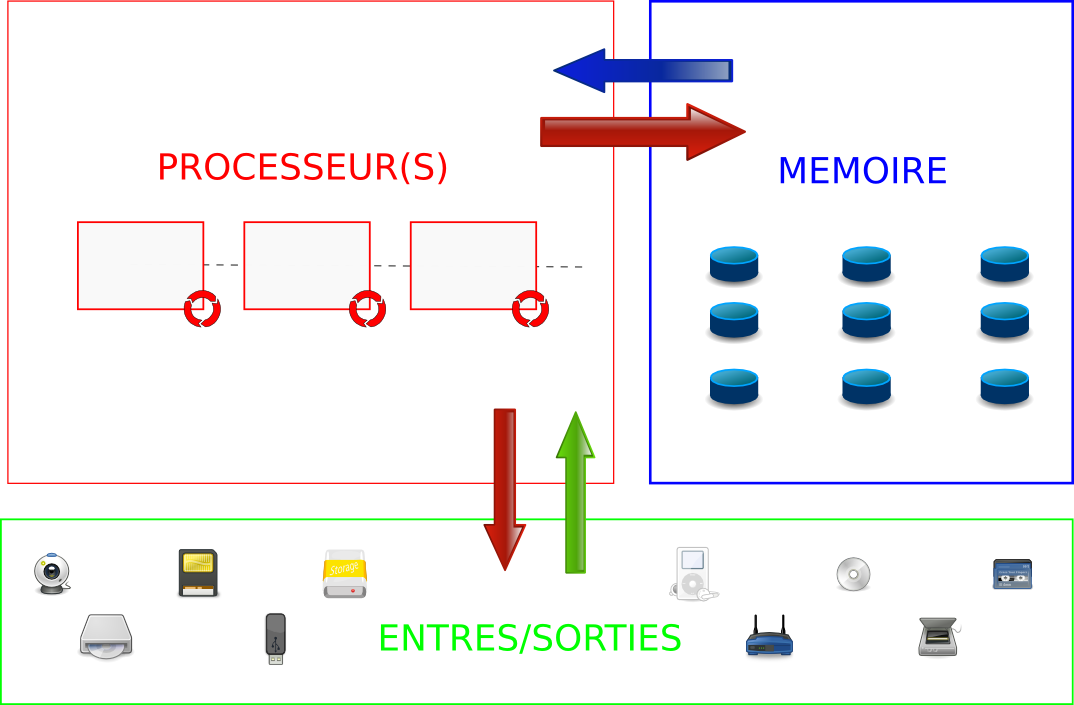
\includegraphics[scale=0.3]{img/cpu-schematics.png}
   \end{center}
  \end{frame}
}

\ifbook{
    \mysubsubsection{Rôle du système d'exploitation}

    \paragraph{} Encore une fois de manière très schématique, et surtout en restant pertinent par
    rapport au thème du cours, le \textit{Middleware}, nous allons maintenant brièvement évoquer le
    rôle du système d'exploitation.

    \paragraph{} En repartant de ce que nous venons de détailler sur le fonctionnement d'un
    ordinateur, plusieurs points peuvent rapidement être gênants. Le principal est que le processeur
    n'exécute qu'un seul programme à la fois, donc tel quel, une seule application peut s'exécuter
    sur un ordinateur à la fois.

    \paragraph{} Le système d'exploitation est une couche logicielle qui va permettre aux programmes
    s'exécutant sur l'ordinateur de se partager les ressources mises à disposition par l'ordinateur
    (processeur, mémoire, périphériques de stockage,...). En outre, le système d'exploitation va
    jouer le rôle d'arbitre entre ces différents programmes, leur attribuant chacun à leur tour un
    certain temps d'utilisation de ces ressources.

    \paragraph{} Ainsi, c'est grâce aux systèmes d'exploitation que de multiples programmes vont
    pouvoir s'exécuter en \textbf{parallèle} sur une machine, qu'elle possède un ou plusieurs
    processeurs.

    \paragraph{} Il est important de noter qu'aucun ordinateur ne pourra effectuer plus de tâches en
    parallèle que son nombre de processeurs, mais les cycles d'exécutions étant extrêmement courts,
    un seul ordinateur, équipé d'un seul processeur, peut donner l'impression à son utilisateur
    d'exécuter simultanément plusieurs tâches. C'est l'impression que vous donne tous les jours,
    les ordinateurs dédiés à la bureautique que vous utilisez.

    \paragraph{Remarque} On notera aussi au passage qu'un même programme peut lui même se diviser en
    plusieurs processus distincts, s'exécutant aussi en parallèle, selon les règles évoquées juste
    avant. Ainsi, dans la cadre d'un projet \textit{middleware} la question de l'exécution, de
    manière concurrente, de différentes parties de l'application peut se poser... (Nous y
    reviendrons plus loin dans le cours).

    \paragraph{} Le schéma \ref{role-os} (page \pageref{role-os} résume les principales
    fonctionnalités d'un système d'exploitation vis-à-vis des applications qui s'exécutent en son
    sein.

    \begin{figure}[h]
      \begin{center}
        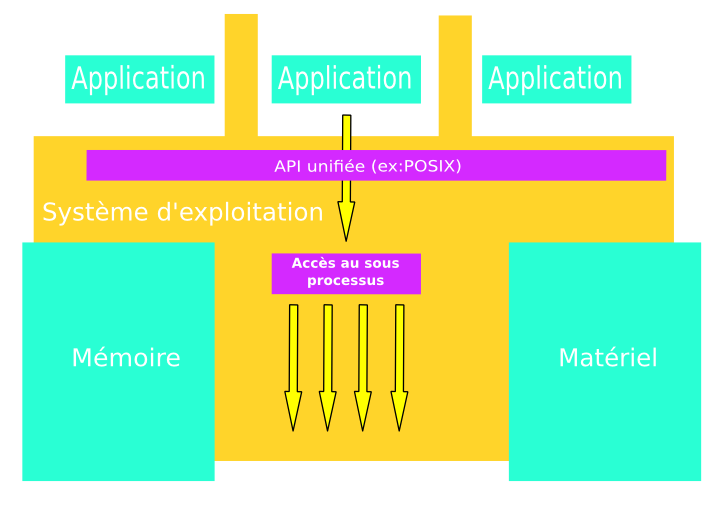
\includegraphics[scale=0.3]{img/operating-system.png}
        \caption{Rôle du système d'exploitation}
        \label{role-os}
      \end{center}
    \end{figure}
}

\ifslide{
  \begin{frame}{Le rôle du système d'exploitation}
    \begin{center}
      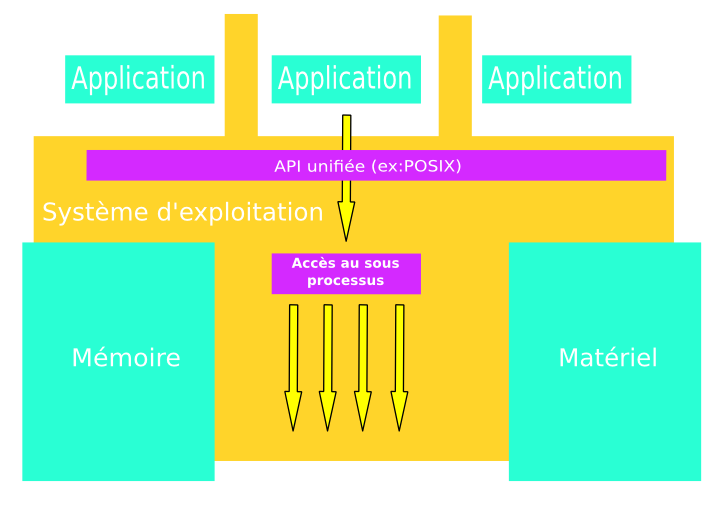
\includegraphics[scale=0.3]{img/operating-system.png}
    \end{center}
  \end{frame}
}

\ifbook{
  \mysubsubsection{Limites physiques d'un ordinateur}
  \paragraph{} Avant d'aller plus loin, arrêtons-nous un instant sur ces notions et sur le système,
  aussi schématique soit-il que nous venons de décrire. Au regard de son fonctionnement, quelles
  limites pouvons-nous déjà percevoir ? Dans quelles conditions, un tel système - l'ordinateur, aura
  des difficultés à effectuer les opérations qu'on lui confie ?

  \paragraph{} Sans surprise, on peut distinguer à peu près autant de limites que de composants
  distingués dans la précédente représentation. Étudions, sommairement, pour chacun d'entre eux les
  limites qu'ils induisent sur l'ordinateur.

  \paragraph{Processeur} La première limite physique d'un ordinateur, qui est pratiquement
  incontournable, est le processeur. Un processeur peut effectuer un certain nombre d'opérations
  dans un certain délai. Dans un système parfaitement optimisé, où tous les autres - assez
  nombreux, nous allons le voir, goulots d'étranglement ont été "neutralisés", cette vitesse
  d'exécution est une limite incompressible : l'ordinateur ne pourra simplement exécuter les
  opérations demandées plus rapidement...

  \paragraph{Parallélisme} Comme évoqué lors de la description du rôle d'un système d'exploitation,
  un ordinateur exécute souvent plusieurs processus à la fois, souvent plus nombreux que son nombre
  de processeurs. Ainsi, il doit passer d'un processus à un autre, à tour de rôle, pour permettre à
  tous de s'exécuter \textit{presque} en parallèle.

  \paragraph{} Il est évident que le passage d'un processus à un autre n'est pas gratuit, et nécessite, de
  la part du système d'exploitation, comme du processeur, un travail supplémentaire qui consiste à
  sauvegarder les données et l'état du processus placé en "pause" et à recharger ceux du processus
  qui "reprend la main".

  \paragraph{} Au bout du compte, si l'ordinateur effectue un nombre de tâches en parallèle
  largement trop grand pour sa capacité, il risque de passer plus de temps à \textbf{changer de
  contexte} entre chaque processus, plutôt qu'à réellement effectuer les opérations qu'on lui
  demande.

  \paragraph{Mémoire} La mémoire à la disposition du processeur impacte généralement grandement la
  vitesse d'exécution. En effet, plus l'ordinateur pourra placer de données en mémoire, plus il
  pourra avoir à sa disposition des résultats intermédiaire et finaux.

  \paragraph{} Illustrons rapidement ce point par un exemple concret. Supposons que l'on confie à
  l'ordinateur de trier un tableau de données, composé d'une seule colonne, par ordre de grandeur
  croissante du contenu de chaque cellule:

  \begin{figure}[h]
    \begin{center}
      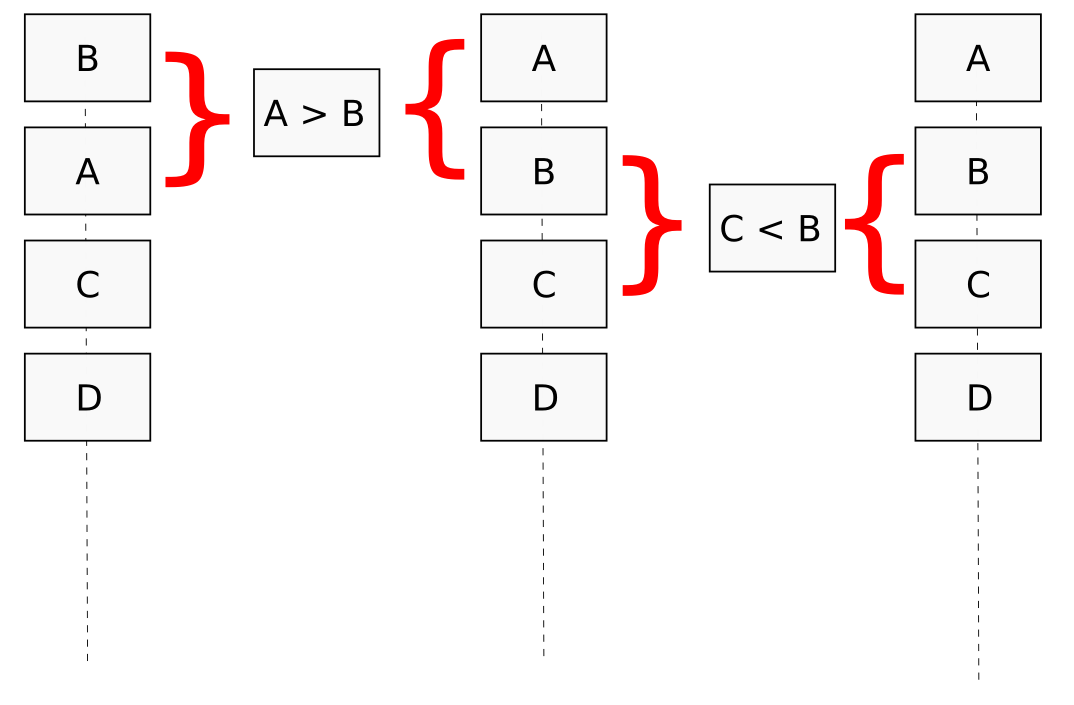
\includegraphics[scale=0.3]{img/exemple-algo.png}
      \caption{Algorithme de tri avec une case mémoire}
      \label{algo-exemple}
    \end{center}
  \end{figure}

}

\ifslide{

  \begin{frame}{Exemple d'algorithme}
    \begin{center}
      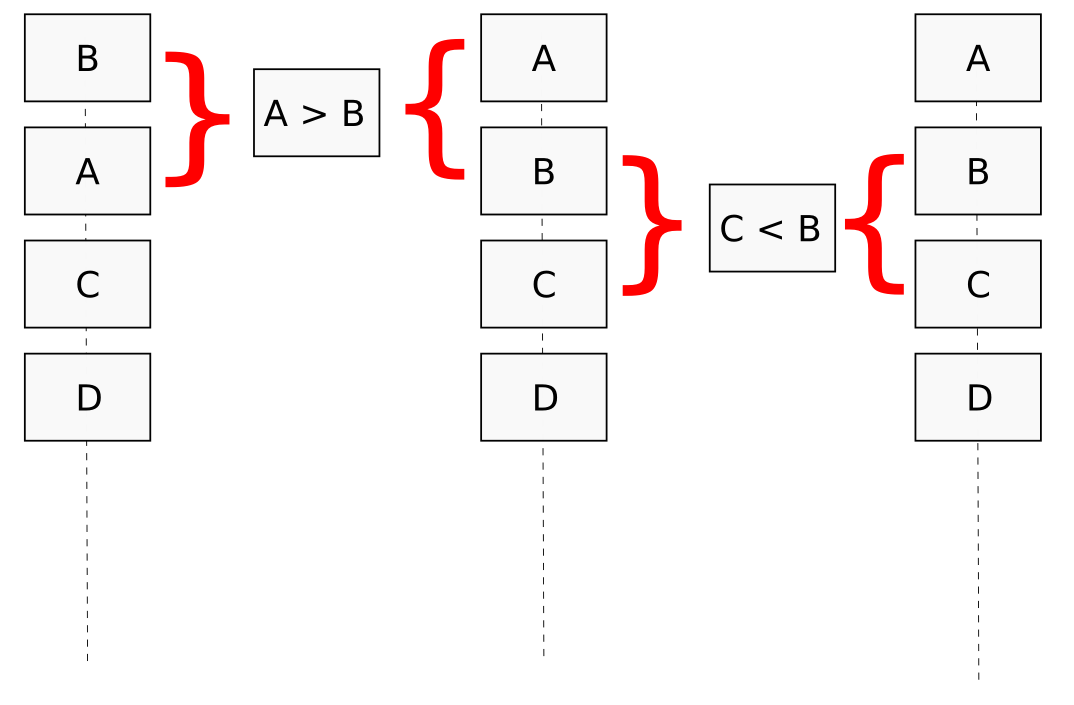
\includegraphics[scale=0.3]{img/exemple-algo.png}
    \end{center}
  \end{frame}
}


\ifbook{

  %TODO:Relire
  \paragraph{} Prenons d'abord comme exemple un ordinateur qui ne pourrait stocker que le contenu 
  des quelques cellules du tableau en mémoire rapide. Il devrait alors lire une cellule, lire la 
  cellule voisine, les comparer et les réécrire dans le bon ordre. Pour cette opération deux lectures
  et deux écritures ont été nécessaire dans une mémoire lente.

  \paragraph{} Si l'ordinateur avait plus de mémoire alors il aurait pu stocker tout le tableau en mémoire rapide et réaliser les opérations de lecture beaucoup plus rapidement avant d'écrire, en une seule fois, le tableau reclassé en mémoire lente

  \paragraph{Remarque} Cet exemple est volontairement grossier afin de souligner l'importance de la mémoire sur la vitesse de traitement. 

  \paragraph{} Si l'ordinateur ne peut stocker qu'un seul résultat intermédiaire, en l'occurrence la
  taille du contenu de la cellule, il ne peut réordonner le tableau qu'en échangeant les cellules
  de positons. En effet, il peut calculer la taille d'une cellule, la stocker, calculer la taille de
  la seconde cellule, la comparer à la précédente et changer l'ordre des deux cellules, si
  nécessaire, puis continuer...

  \paragraph{} Après un laborieux travail, cet \textbf{algorithme}, illustré sur la figure
  \ref{algo-exemple}  (page \pageref{algo-exemple}), sera donc capable de réordonner l'ensemble du
  tableau, mais en effectuant un important nombre d'opérations. À l'inverse, si le processeur est
  libre de placer autant de résultats en mémoire que d'entrées dans le tableau, il pourra se
  contenter de calculer, une fois pour toute, la taille de chaque cellule, puis de les trier de
  manière plus "globale"...

  \paragraph{Remarque} Cet exemple est volontairement très grossier et n'est pas représentatif du
  tout du fonctionnement interne réel d'un ordinateur, ni même de la manière dont le processeur va
  implémenter un algorithme de tri. Néanmoins, sans être l'exemple le plus respectueux des détails
  techniques d'un ordinateur, il illustre de manière très juste l'importance de la mémoire pour la
  réalisation d'opérations au sein d'un ordinateur.

  \paragraph{Entrées/Sorties} Après la mémoire, c'est très certainement les entrées/sorties la
  source de goulot d'étranglement la plus commune au sein d'un ordinateur. Pour bien comprendre
  l'impact de ces dernières sur les performances de l'ordinateur, il suffit de regarder la figure
  \ref{pyramid-io} (page \pageref{pyramid-io} qui décrit, sous forme de pyramide, la vitesse d'accès
  des différentes entrées/sorties, les unes par à rapport aux autres.

  \begin{figure}[h]
    \begin{center}
      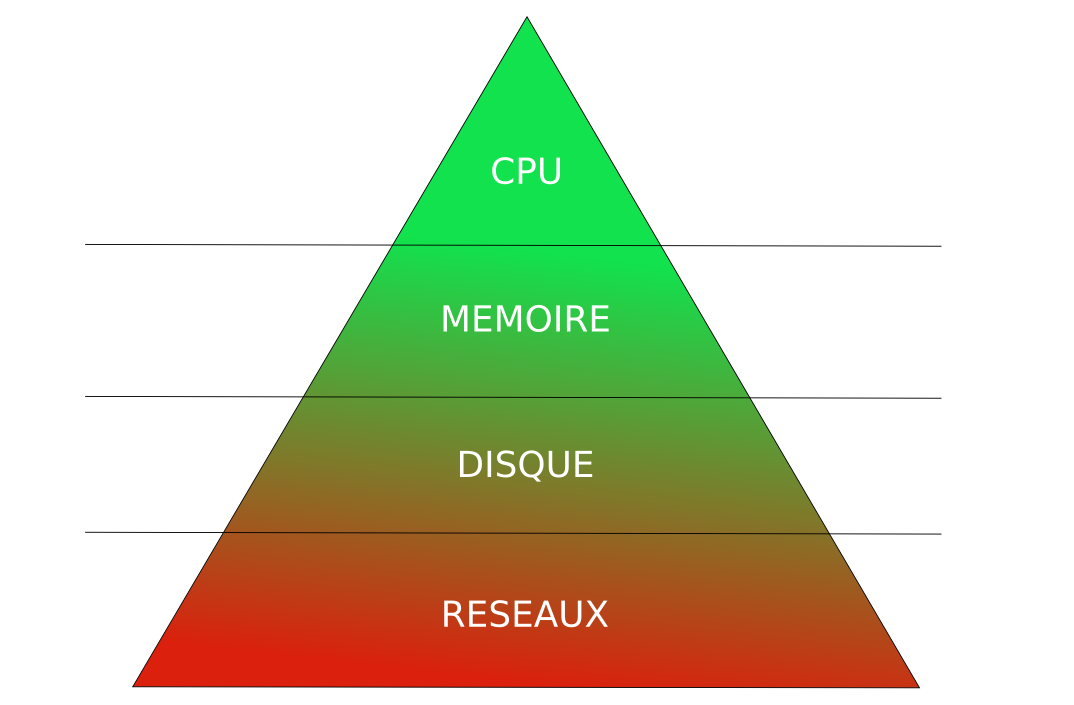
\includegraphics[scale=0.3]{img/pyramid-io.png}
      \caption{Vitesse des entrées/sorties selon les périphériques}
      \label{pyramid-io}
    \end{center}
  \end{figure}

}

\ifslide{
  \begin{frame}{Vitesse d'accès des périphériques}
    \begin{center}
      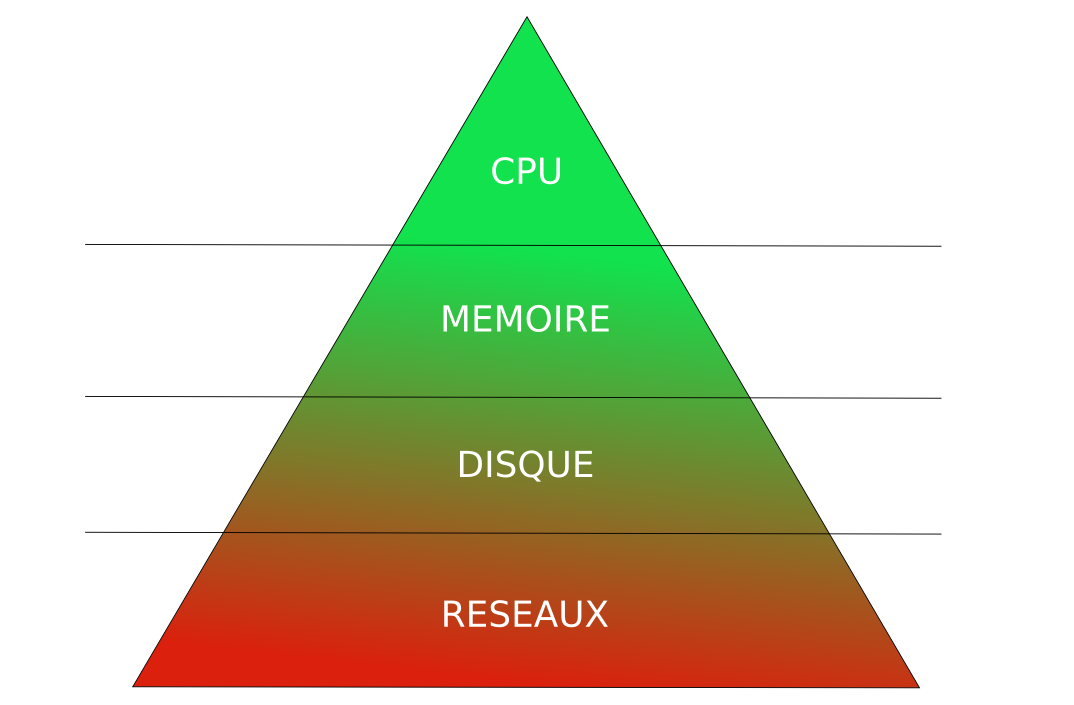
\includegraphics[scale=0.3]{img/pyramid-io.png}
    \end{center}
  \end{frame}
}

\ifbook{

  \paragraph{} À l'étude de ce tableau, il apparaît assez flagrant que si une information nécessaire
  à la bonne exécution du programme est située sur un périphérique inutilement lent (par exemple: sur
  disque dur plutôt qu'en mémoire, sur un serveur distant plutôt que sur le disque dur,...), le
  système en sera ralenti.

  \paragraph{Remarque:} \textit{Ce développement sur les limites physiques d'un ordinateur est volontaire.
  En effet, dans le cadre de la conduite de projet \textit{Middleware}, ces limites seront à
  prendre à compte, dès la conception et l'architecture d'une solution logicielle, pour s'assurer que,
  lors de sa mise en production, le système construit ait une chance de donner les performances
  souhaitées.}

  \paragraph{}\textit{Si des experts techniques sont généralement là pour assister les personnes en charge
  de la conduite, il reste important que ces dernières gardent ses problématiques à l'esprit et soient
  capables d'en discuter avec les susnommés experts...}

}
